\chapter{Topological states in fractal lattices}
\label{ch:fractals}
In the previous chapter, we have shown the importance of internal symmetries and dimensionality in building a classification of different free-fermionic Hamiltonians. Most of the topological phases in distinct symmetry classes are studied by considering clean systems limit, where it is possible to employ the concepts related to the Brillouin zone. However, disordered systems or lattice models without translational symmetries may also host topological states. For instance, quasicrystals, aperiodic systems that posses long-range order~\cite{quasicrystals}, exhibit topological properties which arise from higher-dimensional space in which these structures are truly translational invariant~\cite{PhysRevLett.109.106402}. Several tilings were used to construct quasicrystalline structures hosting topological states protected by the symmetries which are forbidden for conventional crystals, including five- or twelve-fold rotations~\cite{PhysRevLett.124.036803,PhysRevLett.123.196401}. Moreover, topological phases can be realized in completely random point sets~\cite{AmorphTIShenoy2017}. Another interesting example is the so-called statistical topological insulator, where the gapless surface states are immune to Anderson localization as long as the disorder ensemble is invariant under a certain symmetry~\cite{statTI2014}.

Self-similar lattices, in particular fractals~\cite{mandelbrot1983fractal}, also fall into the category of aperiodic systems. Rather than a translational invariance, they posses a scale invariance and are characterized by a Hausdorff dimension $d_{\mathrm{H}$, which is not necessary an integer. A concept of fractals has been extensively studied in the context of condensed matter physics, ranging from spin models defined on fractal lattices~\cite{PhysRevLett.45.855, fractalIsing1998} to the multifractal structure of wave functions at the Anderson metal-insulator transition point~\cite{nakayama2013fractal}. More recent studies covered quantum transport~ \cite{2016:TomadinTransport1} and optoelectronic properties~\cite{2017:YuanOptCond, plasmons} in fractal geometries, localization in deterministic and random fractal lattices~\cite{biblap1, biblap3, 2017:SachaRandFractal}, or defects in regular lattices arranged in a fractal manner~\cite{biblap2}. Progress in the field in not only restricted to theoretical predictions --  artificial fractal structures have been already experimentally realized using focused ion beam epitaxy~\cite{FIBSC}, by depositing atoms on a surface~\cite{Kempkes2019} or assembling molecules~\cite{Shang2015}. 
 
Since it is possible to define quantum states on general graphs, it is important to ask what type of properties a graph must have to host topological states (notably, to define the topology of quantum states, only a notion of locality and the possibility to take a thermodynamic limit are required). Here, we would like to address this question by examining two fractal lattice, Sierpiński carpet (SC) and Sierpiński gasket (or triangle, SG), in a homogeneous magnetic field. Sierpiński carpet and gasket are different in terms of their dimensionality and connectivity properties. Recall, the Hausdorff dimension is given as 
\begin{equation}
d_{\mathrm{H}} = \frac{ \ln A}{ \ln L}
\end{equation}
where $A$ is the covered area of a fractal with linear extend $L$. For SC, $d_H \approx 1.892 \ldots$, while for SG $d_H \approx 1.585$. Another property, ramification number $\mathcal{R}$, is said to be finite if after eliminating a finite number of bonds one can isolate an arbitrarily large part of a system. For SC, $\mathcal{R} = \infty$, while SG has finite ramification $\mathcal{R} = 4$.   

Even though spectral properties of SC and SG were investigated before~\cite{GHEZ19871291,PhysRevB.29.5504, PhysRevLett.49.1194, PhysRevB.60.10054}, topological aspects of the Hamiltonians defined on such lattices remain not fully explored. Authors in Ref.~\cite{2018:BHZ} reported results on BHZ model defined on three distinct fractal geometries, while in Ref.~\cite{PaiFractal2019} construction of spinless chiral $p-$ and $p +ip-$wave superconductors on SC and SG was discussed. Understanding the bulk-boundary correspondence in such systems is problematic as well as there is no sharp distinction between the bulk and edge. It was found that the edge states in SC corresponding to non-zero $\sigma_{xy}$ are always present for a finite field strength and stable as one approaches the thermodynamic limit~\cite{EdgesFremling2020}. On the other hand, the Hall conductivity is not always proportional to the Chern number~\cite{KatnelsonFractal2020}

As a final motivation to investigating Hamiltonians on fractals is related to the fractons. Fractonic topologically ordered models host fractionalized point-like excitations, fractons, which are immobile. In some of them (called type-II) operators that create excitations have support on a fractal subset of the three-dimensional lattice.

\section{Model}
\label{sec:frac_model}
We investigate the lattice regularization of two aforementioned geometries (consult Fig.~\ref{fig:lattice}). Complex fractal pattern can be generated by the iterative procedure in which the system size increases with every step, but the distance between lattice sites remains the same. Such setting is most relevant to potential experiments on a nanoscopic scale as it introduces a natural cutoff. In order to construct the carpet, we start with a simple square lattice with $L (n) = 3^n$ sites along the outer edge, where $n$ is an iteration step. Then, in every step $n$, $ \left( 1 - ( 8 /9 )^n \right) \cdot 9^n$ lattice sites are removed. From the Pascal's triangle modulo $m$ (with $m$ being a prime number) embedded in a triangular lattice having $2^n + 1$ rows, it is possible to obtain a series of gasket-like lattices with $d_H = 1 + \log_m \left( \frac{m + 1}{2} \right)$ and the case of $m = 2$ corresponds to SG.

\begin{figure}[h]
\centering
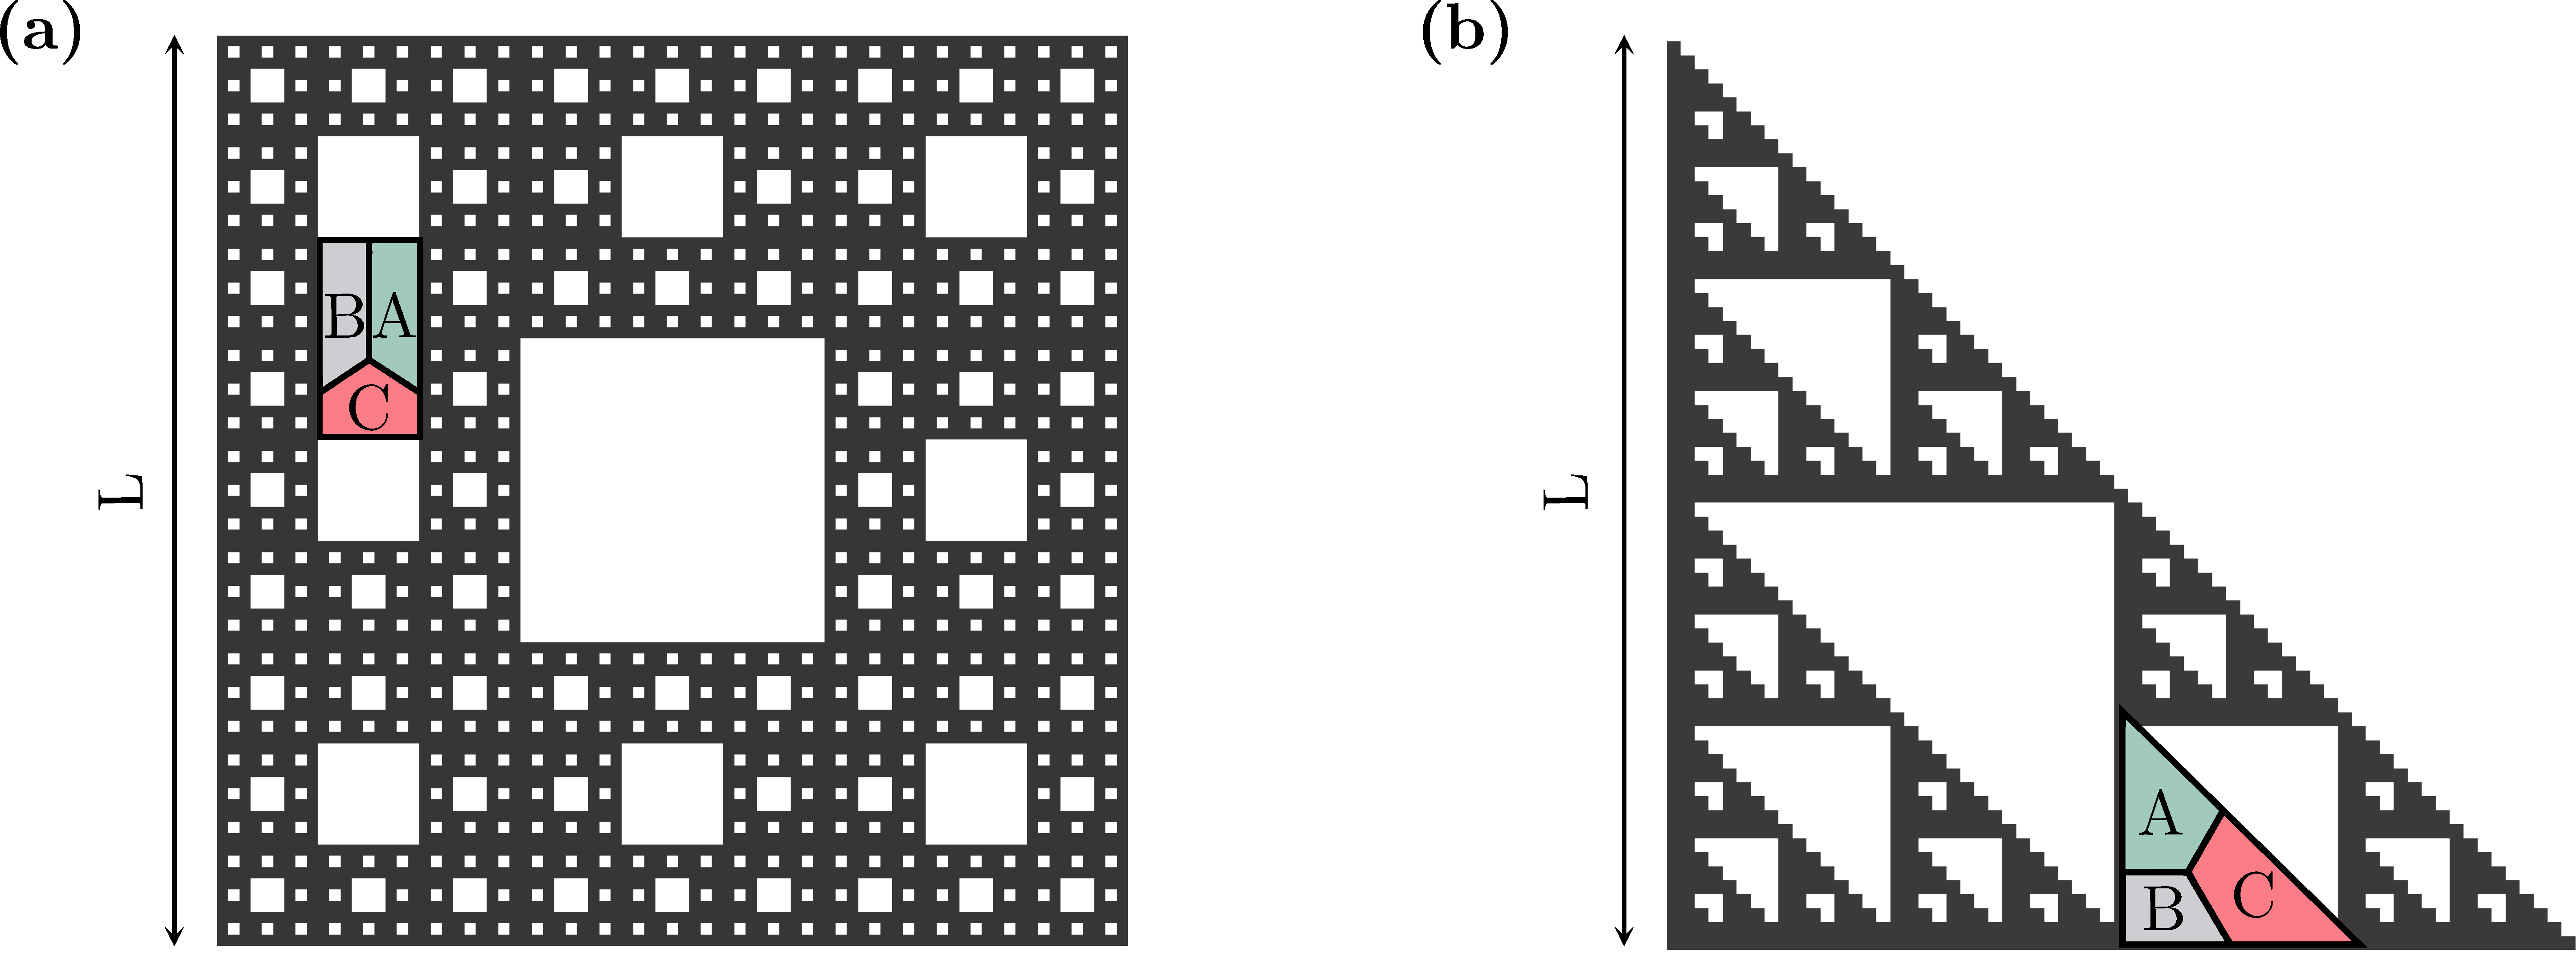
\includegraphics[width=0.95\columnwidth]{frac_lattice.pdf}
\caption{\textbf{Fractal lattices: (a)} the forth iteration of the Sierpiński carpet with $L = 81$ and \textbf{(b)} the sixth iteration of the Sierpiński gasket with $L = 65$. Black squares depict the lattice sites which are kept from underlying regular square (in case of carpet) and triangular (gasket) lattices. Summation regions used in real-space Chern number calculations are labeled with A, B, C.}
\label{fig:lattice}
\end{figure}
In the following, we consider a tight-binding Hamiltonian describing non-interacting spinless fermions exposed to a perpendicular magnetic field 
\begin{equation}
H = -t  \sum_{\langle i, j \rangle} e^{\textnormal{i} A_{ij}} c^{\dagger}_i c_j + \mathrm{h.c.},
\label{eq:frac_ham}
\end{equation}
where $i$ labels lattice sites. The hopping integral $t$ between nearest-neighbors is the only energy scale in the model and it is set to $t = 1$. Magnetic field is taken into account by employing Peierls substitution which gives rise to the phase factors $A_{ij} = \int_i^j \mathbf{A} \cdot d \mathbf{r}$, with $\mathbf{A}$ being the vector potential satisfying relation $\mathbf{B} =  \nabla \times \mathbf{A}$. We assume that the magnetic field is homogeneous in the two-dimensional space in which the fractal lattice is embedded. The magnetic flux per smallest element of lattice-regulated versions of carpet and gasket (that is, the smallest square in the SC and the smallest triangle for the SG) is chosen to be $\Phi$,  a fraction $\alpha$ of the flux quantum $\Phi_0$. In units where $\hbar = e = 1$, $\Phi_0 = 2 \pi$, hence $\Phi  /  \Phi_0 = \alpha$. The phase factors distribution is presented in Fig.~\ref{fig:flux_distr}.

\begin{figure}
\centering
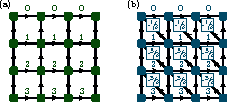
\includegraphics[width=0.9\columnwidth]{frac_flux.pdf} 
\caption{\textbf{Vector potential gauge choice:} Phase distribution on $4 \times 4$ \textbf{(a)} square and \textbf{(b)} triangle lattices with open boundary conditions. $A_{ij}$ phase between sites $i$ and $j$ is equal to the number shown above the bond in $2 \pi$ units. A phase acquired with the respect to the direction pointed by arrows has a positive sign.}
\label{fig:flux_distr}
\end{figure}


\section{Spectral properties}
\label{sec:frac_spectral}
Firstly, let us focus on the energy spectra obtained by diagonalizing the Hamiltonian given in Eq.~\eqref{eq:frac_ham} for different values of the magnetic flux. In Fig.~\ref{fig:frac_spect} (a, d), we show the density of states (DOS) for the SC at iteration $n = 4$ and the SG at iteration $n = 6$ with open boundary conditions. Discrete sets of energy levels $E_\lambda$ are smoothed using a Gaussian function $f(E, \alpha) = \sum_{\lambda} \exp  \left\{ - \left[ E - E_{\lambda} (\alpha) \right]^2 / \eta \right\}$ with broadening $\eta = 0.001$. As in case of regular lattices, a presence of magnetic field gives rise to the self-similar spectrum in the energy-flux plane known as Hofstadter's butterfly~\cite{1976:Hofstadter}. The spectrum of the SC (see Fig.~\ref{fig:frac_spect}~(a)) is reflection-symmetric with respect to the $E = 0$ and the $\alpha = 1/2$ lines due to a chiral symmetry of the Hamiltonian on this bipartite lattice. Two finite gaps of maximal extend in energy $\sim 0.1$ are observed for small range of the flux around $\alpha = 1/4, \, 3/4$ and $E = 0$. Regions of low DOS (which are fully gapped if periodic boundary conditions are assumed) host states with distinct localization properties, which are discussed in more details in Section~\ref{sec:frac_edgemodes}. Fig.~\ref{fig:frac_spect}~(d) shows the spectrum of the SG, which has only a point-inversion symmetry about $\alpha=1/2$ and $E=0$, and exhibits various fully gapped regions. Large DOS appears around two points: $\alpha = 1/4$, $E \approx 1.4$ and symmetry-related $\alpha = 3/4$, $E \approx -1.4$. It is known that at zero flux the spectrum is fractal and the energy levels are macroscopically degenerated~\cite{PhysRevB.28.3110}; introducing a finite field leads to lifting this degeneracy.

\begin{figure}[H]
\centering
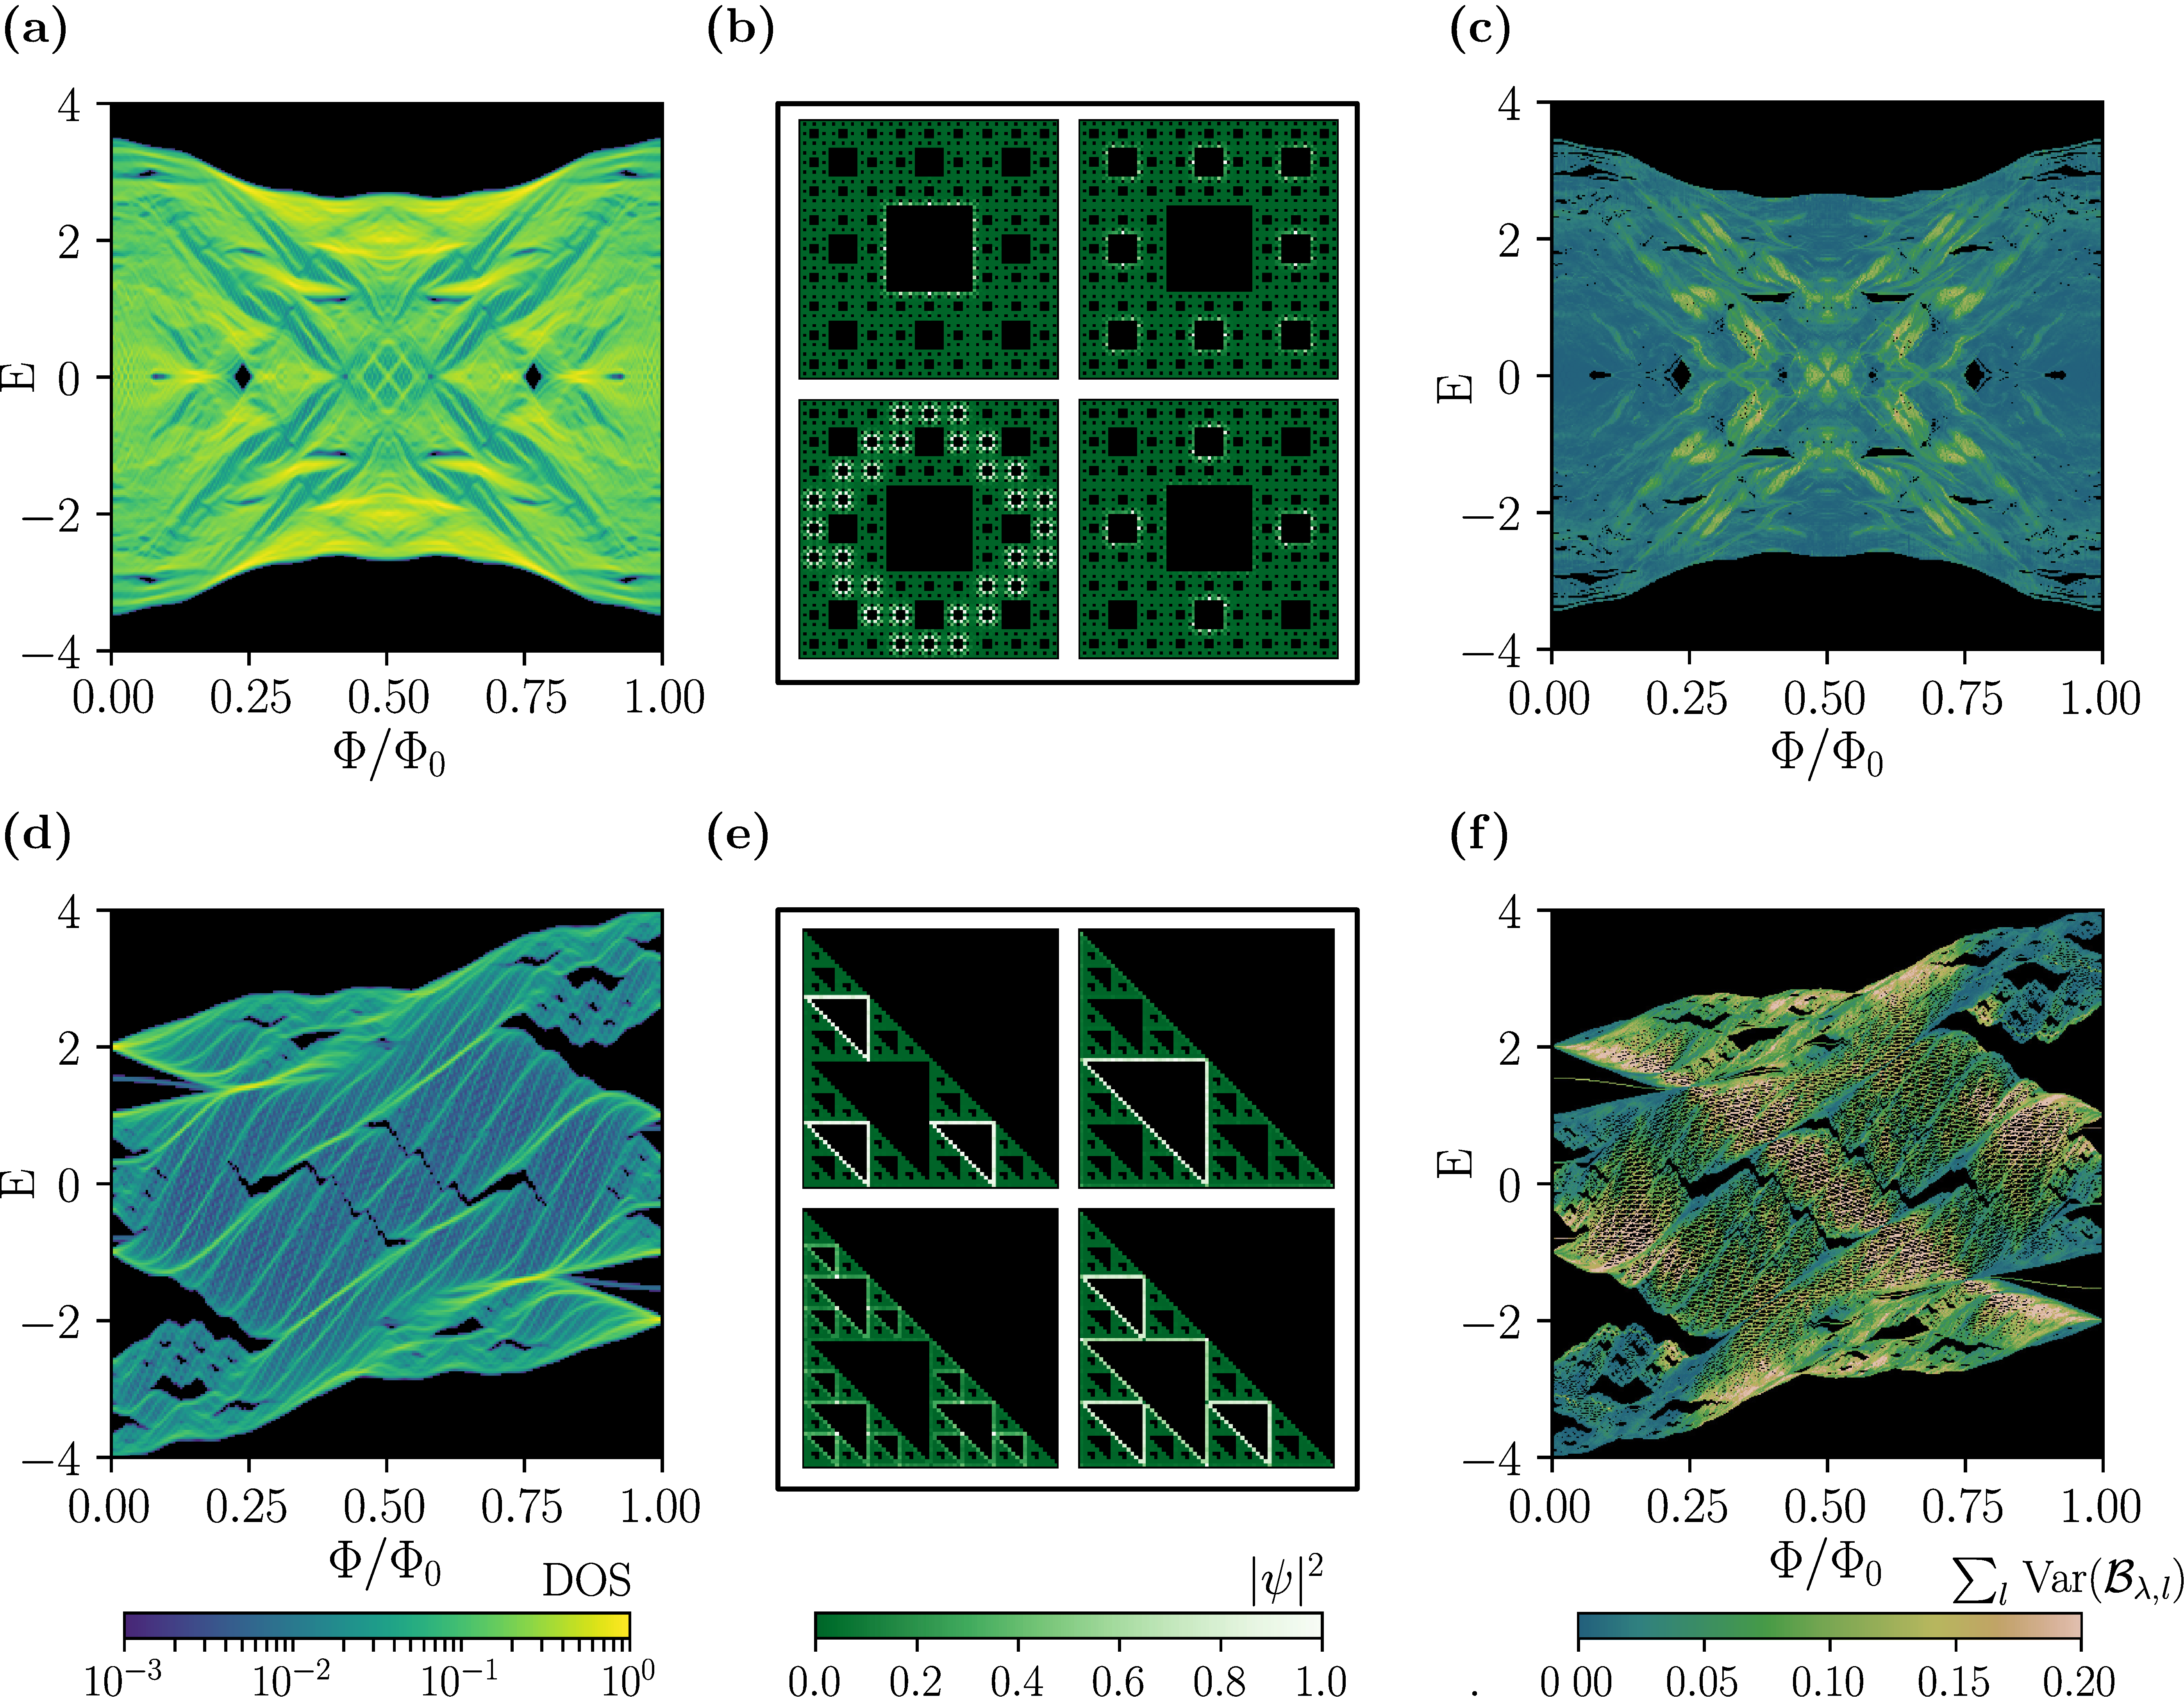
\includegraphics[width=1.05\textwidth]{frac_spectra.pdf} 
\caption{\textbf{Spectral and eigenstate localization properties:} \textbf{(a, d)} Density of states in the energy-flux plane, \textbf{(b, e)} localization of the eigenstates, and \textbf{(c, f)} edge-locality marker. Low DOS regions are represented by dark blue color. Two energy gaps at $E = 0$ are seen for SC, while the energy spectrum of SG exhibits numerous gaps. Representative electronic densities at time-reversal symmetric point ($\alpha = 1/2$) around $E = 0$ are presented in \textbf{(b, e)} and the color scale corresponds to the square modulus $| \psi_i|^2$ of the wave function normalized by its maximum value. $\mathcal{B}_{\lambda, l}$ marker shown in \textbf{(c, f)} quantifies the changes in localization properties between consecutive eigenstates at fixed flux. Parts of the spectra with smaller density are associated with largely varying values of edge-locality marker.}
\label{fig:frac_spect}
\end{figure}


\section{Edge modes}
\label{sec:frac_edgemodes}
A striking feature of a conventional integer quantum Hall setup is the existence of protected edge modes. As a distinction between bulk and boundaries in fractal lattices is not sharp, it is crucial to investigate the localization eigenstate properties more carefully. Previous studies of fractal lattices suggested~\cite{supp1, supp2} that introducing a magnetic field leads (on average) to delocalization of eigenstates. This observation can be confirmed by computing inverse participation ratio (IPR)
\begin{equation}
I_{\psi} = \frac{\sum_i | \psi_i |^4}{\left(\sum_i  |\psi_i |^2 \right)^2}, 
\label{eq:ipr}
\end{equation}
for any wavefunction expandable in a site basis $\ket{\psi} = \sum_i \psi_i \ket{i}$. IPR takes values between 1 and the inverse of the number of sites $N$, where 1 corresponds to perfect localization at one site and $1/N$ to evenly distributed weights over all lattice sites. At zero flux $\alpha = 0$, the distribution of IPRs is peaked close to the inverse of the number of sites belonging to the edges of the second-smallest squares or triangles. For a finite field, the distribution of IPRs shifts to smaller, i.e., more delocalized values. This effect is more apparent for the SC compared to the SG.

\begin{figure}[H]
\centering
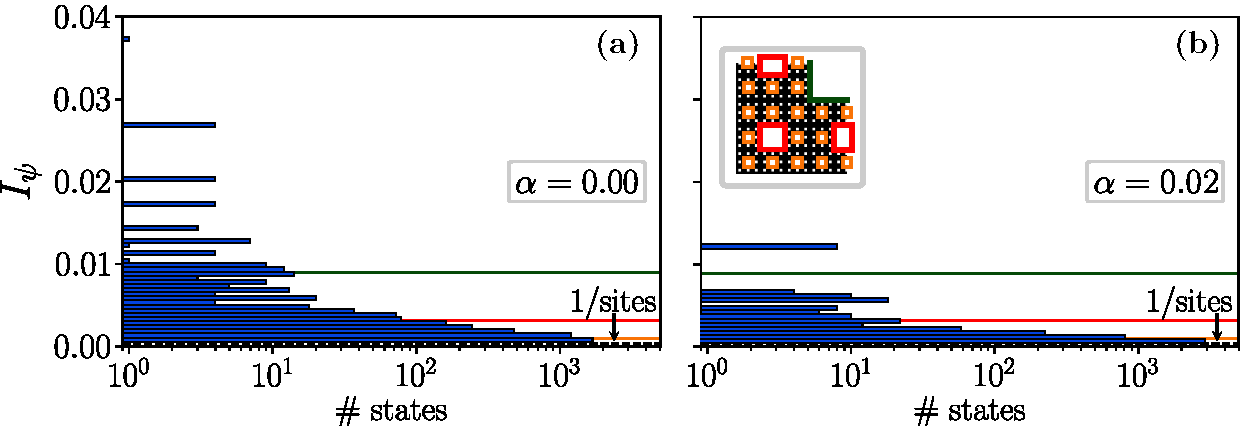
\includegraphics[width = 1.05\columnwidth]{frac_iprSC.pdf}
\caption{\textbf{Distribution of IPR for Sierpiński carpet:} at \textbf{(a)} $\alpha = 0$ and \textbf{(b)} $\alpha = 0.02$. Inset presents a closeup of carpet with internal edges of different hierarchies marked with different colors.}
\label{fig:IPR_SC}
\end{figure}

\begin{figure}[H]
\centering
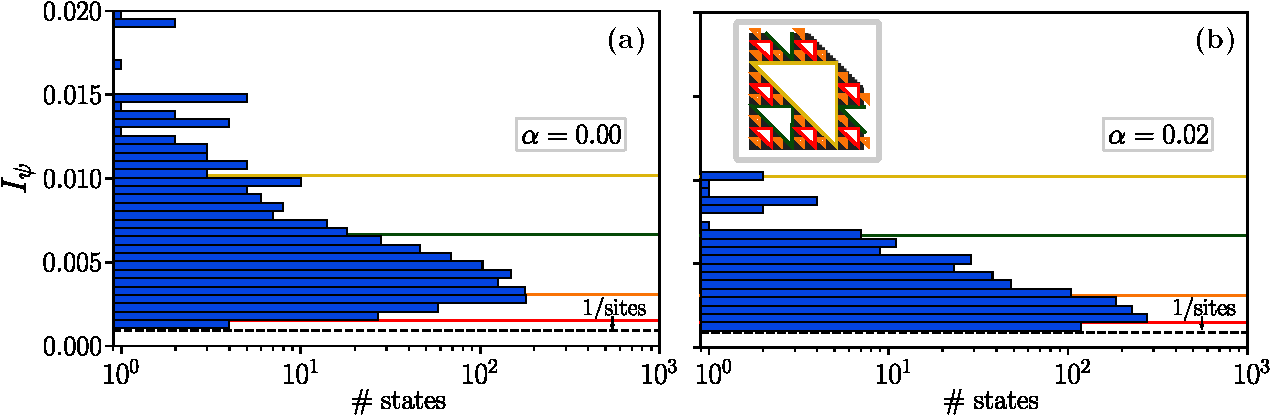
\includegraphics[width = 1.05\columnwidth]{frac_iprSG.pdf}
\caption{\textbf{Distribution of IPR for Sierpiński gasket:} at \textbf{(a)} $\alpha = 0$ and \textbf{(b)} $\alpha = 0.02$. Inset displays a closeup of gasket with highlighted edges of different hierarchies.}
\label{fig:IPR_SG}
\end{figure}

Remarkably, by contrasting the case of zero and non-zero magnetic field, we observe an intriguing change in the character of the most localized states. Fig.~\ref{fig:frac_spect}~(b, e) show the electronic densities for the eigenstates at the time-reversal symmetric point ($\alpha = 1/2$) around zero energy. States are sharply localized at the internal edges of the fractal at different levels of the hierarchy and they can be found in very close spectral proximity to one another in various places of the phase diagram at finite magnetic field. Conversely, at zero magnetic field, the most localized states are usually not supported on internal edges. To quantify the degree of localization, we compute edge-locality marker defined as
\begin{equation}
\mathcal{B}_{\lambda, l} = \sum_{i \in \mathcal{E}_l} | \psi_{\lambda,i} |^2, 
\label{eq:edgemarker}
\end{equation}
where $\braket{i | \psi_{\lambda}} = \psi_{\lambda,i} $ and the summation is taken over the edges $\mathcal{E}_l$ of all internal triangles or squares at level $l$ of the hierarchy. Hence, $\mathcal{B}_{\lambda, l}$ measures how much an eigenstate $\ket{\psi_{\lambda}}$ with an energy $E_{\lambda}$ has a support on different edges of hierarchy level $l$. With every state $\ket{\psi_{\lambda}}$ , we associate a set of $\mathcal{B}_{\lambda, l}$ for $l = 0, \ldots, n$. In order to detect where in the phase diagram the localization properties are varying at most, we compute the variance for each entry of the set $\mathcal{B}_{\lambda, l}$ across three states with energies $E_{\lambda - 1}$, $E_{\lambda}$ and $E_{\lambda+1}$, and sum these variances over $l$. Results shown in Fig.~\ref{fig:frac_spect}~(c, f) indicate that sharp changes in eigenstate localization appear mostly in the low DOS regions, thus we can interpret these regions as made of edge-like states at various levels of the fractal hierarchy.

\begin{figure}[h]
\centering
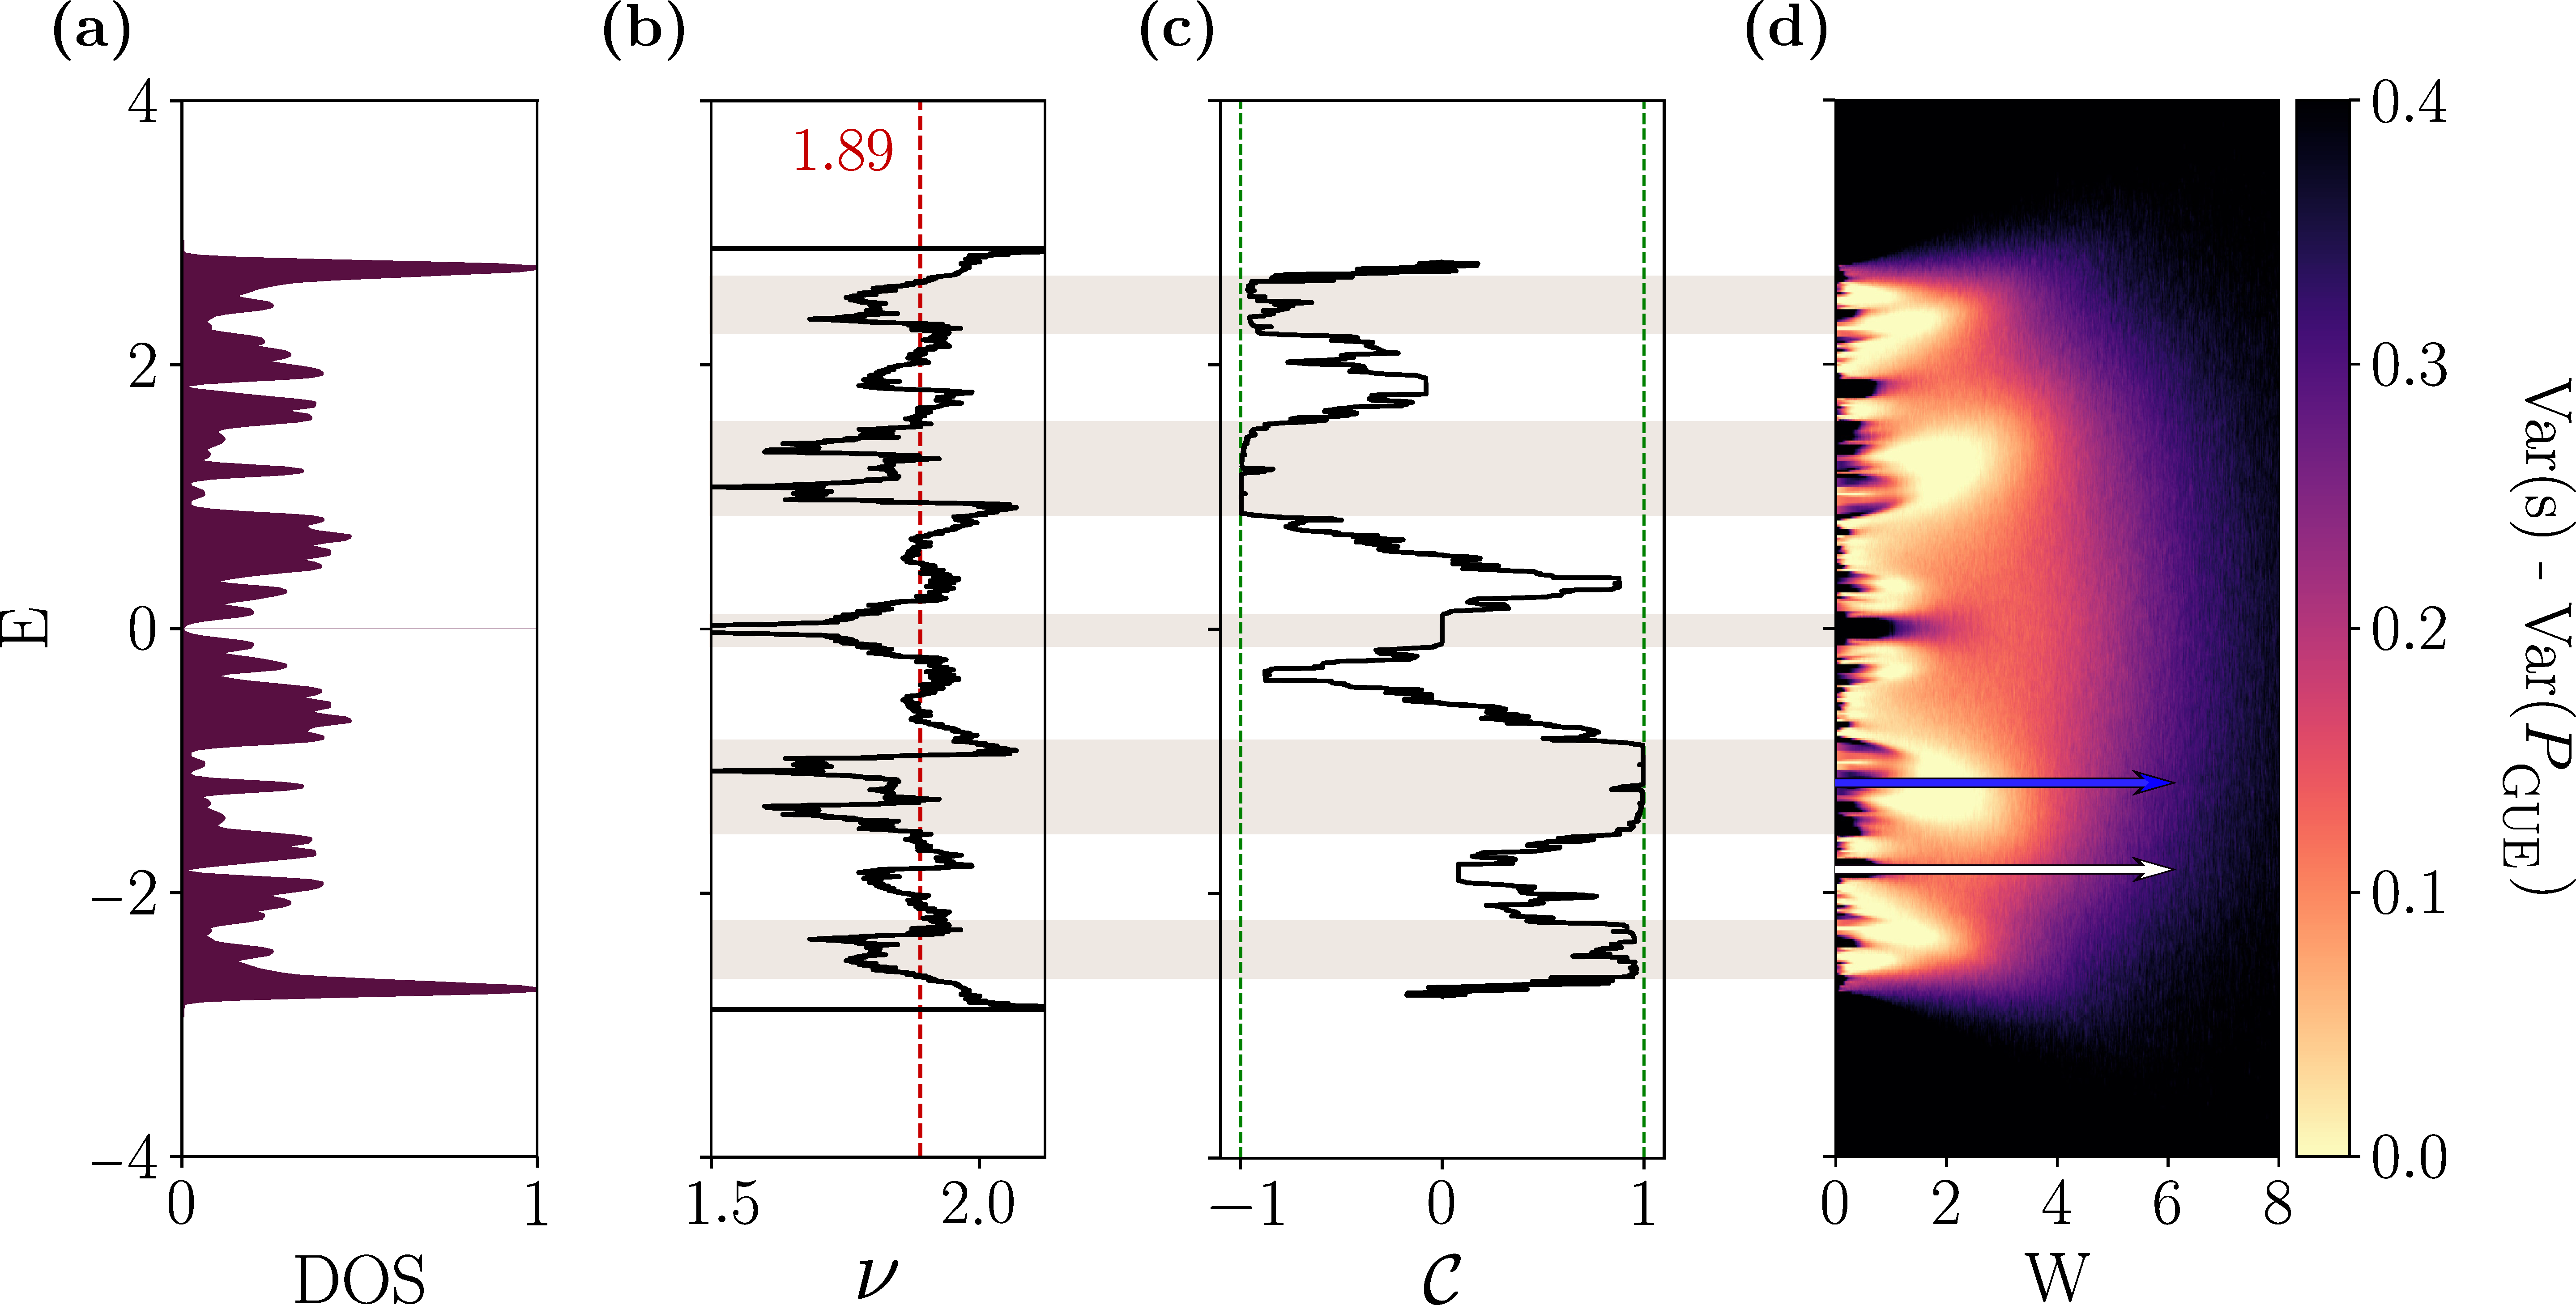
\includegraphics[width=0.95\textwidth]{frac_SC.pdf} 
\caption{\textbf{Detecting topological properties of Sierpiński carpet at fixed flux $\alpha = 1/4$: (a)} density of states, \textbf{(b)} scaling exponent $\nu$ of the DOS with system size, \textbf{(c)} the Chern number as a function of $E$ and  \textbf{(d)} variance of level spacings in the energy-disorder strength plane. Grey rectangles are drawn to guide the eye. We identify energy gaps to be trivial. Regions with quantized values of the Chern number close to 1 are separated by a delocalized state from the Anderson insulator limit (see blue arrow in \textbf{(d)}), which is a feature of quantum Hall states. This is in contrast to a direct transition to a fully localized phase for states carrying zero Chern number as a function of $W$ (white arrow in \textbf{(d)}). States with $\mathcal{C} \neq 0$ are characterized by a DOS scaling exponent $\nu$ smaller than $d_{H}$ in \textbf{(b)}.}
\label{fig:frac_SC}
\end{figure}

\begin{figure}[h]
\centering
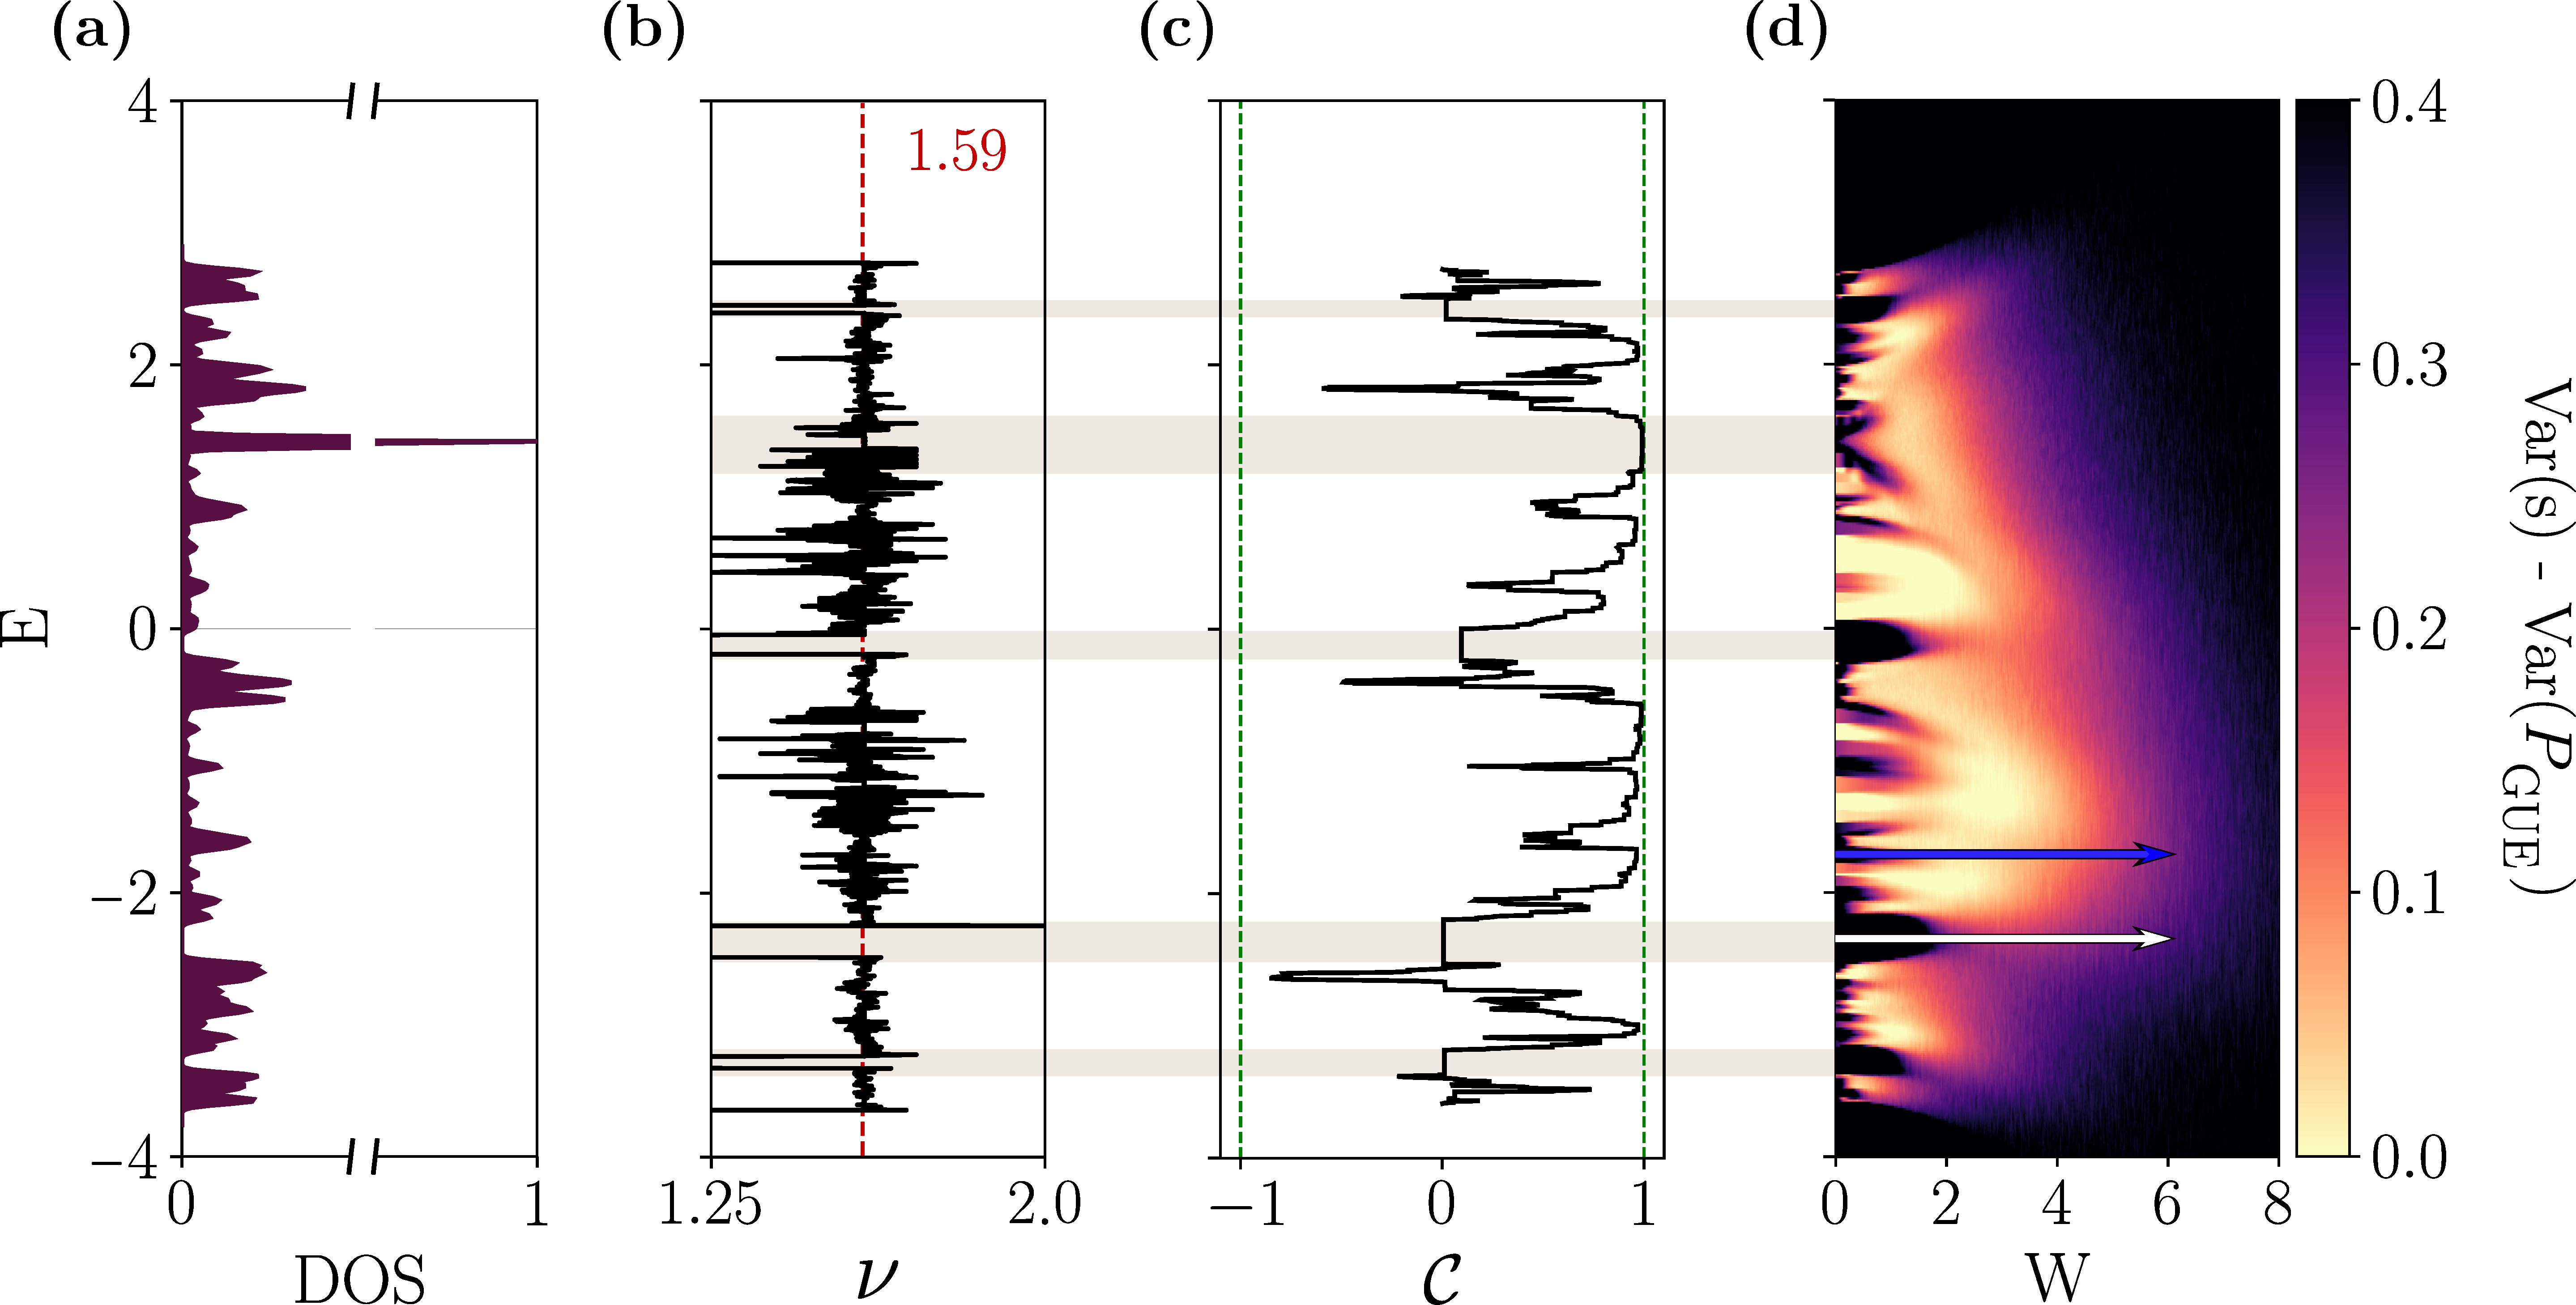
\includegraphics[width=0.95\textwidth]{frac_SG.pdf} 
\caption{\textbf{Detecting topological properties of Sierpiński gasket at fixed flux $\alpha = 1/4$: (a)} density of states, \textbf{(b)} scaling exponent $\nu$ of the DOS with system size, \textbf{(c)} the Chern number as a function of $E$ and \textbf{(d)} variance of level spacings in the energy-disorder strength plane. Similar to SC, spectral gaps are also topologically trivial. Quantization of the Chern number is less pronounced, but the levitation and pair annihilation mechanism is still observed (see \textbf{(d)}).}
\label{fig:frac_SG}
\end{figure}

\section{Real-space formulation of topological invariants}

Due to lack of translational invariance, it is not possible to compute the Chern number directly from the bundle of Bloch occupied bands. Instead, we employ the real-space formula for the Chern number based on an antisymmetric product of projection operators~\cite{KITAEV20062}
\begin{equation}
\mathcal{C} = 12 \pi \mathrm{i} \sum_{j \in A} \sum_{k \in B} \sum_{l \in C} \left( P_{jk} P_{kl} P_{lj} - P_{jl} P_{lk} P_{kj} \right),
\label{eq:chern_real}
\end{equation}
where $P =  \ket{\psi} \bra{\psi}$ is the projection operator onto occupied subspace with respect to a given Fermi level $E_F$ and $j, \, k, \, l$ label the lattice sites in three distinct neighboring sectors $A$, $B$ and $C$ arranged in a counterclockwise manner (consult Fig.~\ref{fig:lattice}). As a remark, for a translationally invariant case Eq.~\ref{eq:chern_real} reduces to
\begin{equation}
\mathcal{C} = 2 \pi \mathrm{i} Tr \left( P \left[ [X, P], [Y, P] \right] \right)
\label{eq:chern_real_translational}
\end{equation}
with $X$ and $Y$ being the operators of $x$ and $y$ coordinates, respectively, and the trace is taken over the unit cell.

The sum in Eq.~\eqref{eq:chern_real} should converge to an integer, when the summation region is large enough. If $\mathcal{C}$ is indeed quantized, it becomes then independent of the detailed choice of $A$, $B$, $C$ in the limit of where the number of sites in each part goes to infinity. Using the SC as an example, in Fig.~\ref{fig:ChernScaling} we show how a real-space patch choice affects the quantization of $\mathcal{C}$. We compute $\mathcal{C}$ while varying the distance $R$ between the center and the corners of the patch that makes up $A$, $B$, $C$ and keeping the aspect ratio of rectangle constant. When the summation region is too small or too large (close to the size of the entire system), $\mathcal{C}$ is far from a non-zero quantized value as expected. We focus on two Fermi levels, $E_F = -1.2$ and $E_F = -1.0$, which correspond to spectral regions with less and more quantized $\mathcal{C}$, respectively. For $E_F = -1.0$, $\mathcal{C}$ is very close to 1 over a large range of $R$. Conversely, for $E_F = -1.2$, where $\mathcal{C}$ is not quantized, a strong $R$-dependence is found.

Figs.~\ref{fig:frac_SC}~(d), \ref{fig:frac_SG}~(d) present $\mathcal{C}$ as a function of the Fermi energy $E$ at fixed value of flux $ \alpha =1/4$ for the $n=4$ iteration of SC and the $n=6$ iteration of the SG with a patch size corresponding to the most robust results. We arrive at following conclusions: (i) All fully gapped regions of the spectrum, for both lattices, carry $\mathcal{C}=0$, (ii) low DOS regions for the SC in Fig.~\ref{fig:frac_spect}~(a) are associated with stable plateaus $\mathcal{C} \sim \pm 1.0$ (for a wide range of energies $E = -1.5 \ldots - 0.9$ and $E = 0.9 \ldots 1.5$), as well as less quantized regions with $\mathcal{C} \sim \pm 0.96$ ($E = -2.6\ldots -2.5$ and $E = 2.5\ldots 2.6$). Deviations from quantized Chern numbers are observed when the DOS is enhanced, for example around $E = -1.2$ and $E = 1.2$. (iii) Identification of non-trivial regions for the SG is less clear, yet a plateau from $E = 1\ldots 1.6$ converges to $\mathcal{C} \sim 1.0$. 

It is not obvious whether for fractals $\mathcal{C}$ tends to quantized values for almost all energies in the thermodynamic limit, that is the deviation from quantized $\mathcal{C}$ is solely due to finite-size effects. Because of exponential increase in size for every iteration, performing systematic finite-size studies remains challenging. To discuss the connection between the DOS and the Chern number,  we calculate the number of states at fixed $\alpha$ averaged over an energy interval $[\epsilon - \delta,\, \epsilon + \delta]$ (with $\delta = 0.1$ for the SC and $\delta = 0.05$ for the SG) for different system sizes, and compute the average scaling exponent $\nu$ of the number of states in that energy range with system size. On average, $\nu$ equals the Hausdorff dimension $d_{\mathrm{H}}$. In Fig.~\ref{fig:frac_SC}~(b) that for the SC regions with (nearly) quantized Chern number consistently show scaling with $\nu < d_{\mathrm{H}}$. This indicates that the normalized DOS would scale to zero in the thermodynamic limit in regions with quantized Chern number. For the SG, the situation is less clear except in regions of trivial Chern number where no states are found (see Fig.~\ref{fig:frac_SG}~(b)). 


%\subsection*{Bott index}
%To use the Bott index, which measures the commutativity of the projected position operators. Algorithm for computing the Bott index~\cite{BottIdx}.
%\begin{equation}
%\begin{aligned}
%U &= P e^{i 2 \pi X} P \\ 
%V &= P e^{i 2 \pi Y} P
%\end{aligned}
%\end{equation}
%where $X, Y$ are the coordinates, rescale to fit the interval $[0, 1)$.
%\begin{equation}
%B = \frac{1}{2 \pi} Im \left( Tr [ \log (V U V^{\dagger} U^{\dagger} ) ] \right)
%\end{equation}
%which requires to take a logarithm of a matrix.

\begin{figure}
\centering
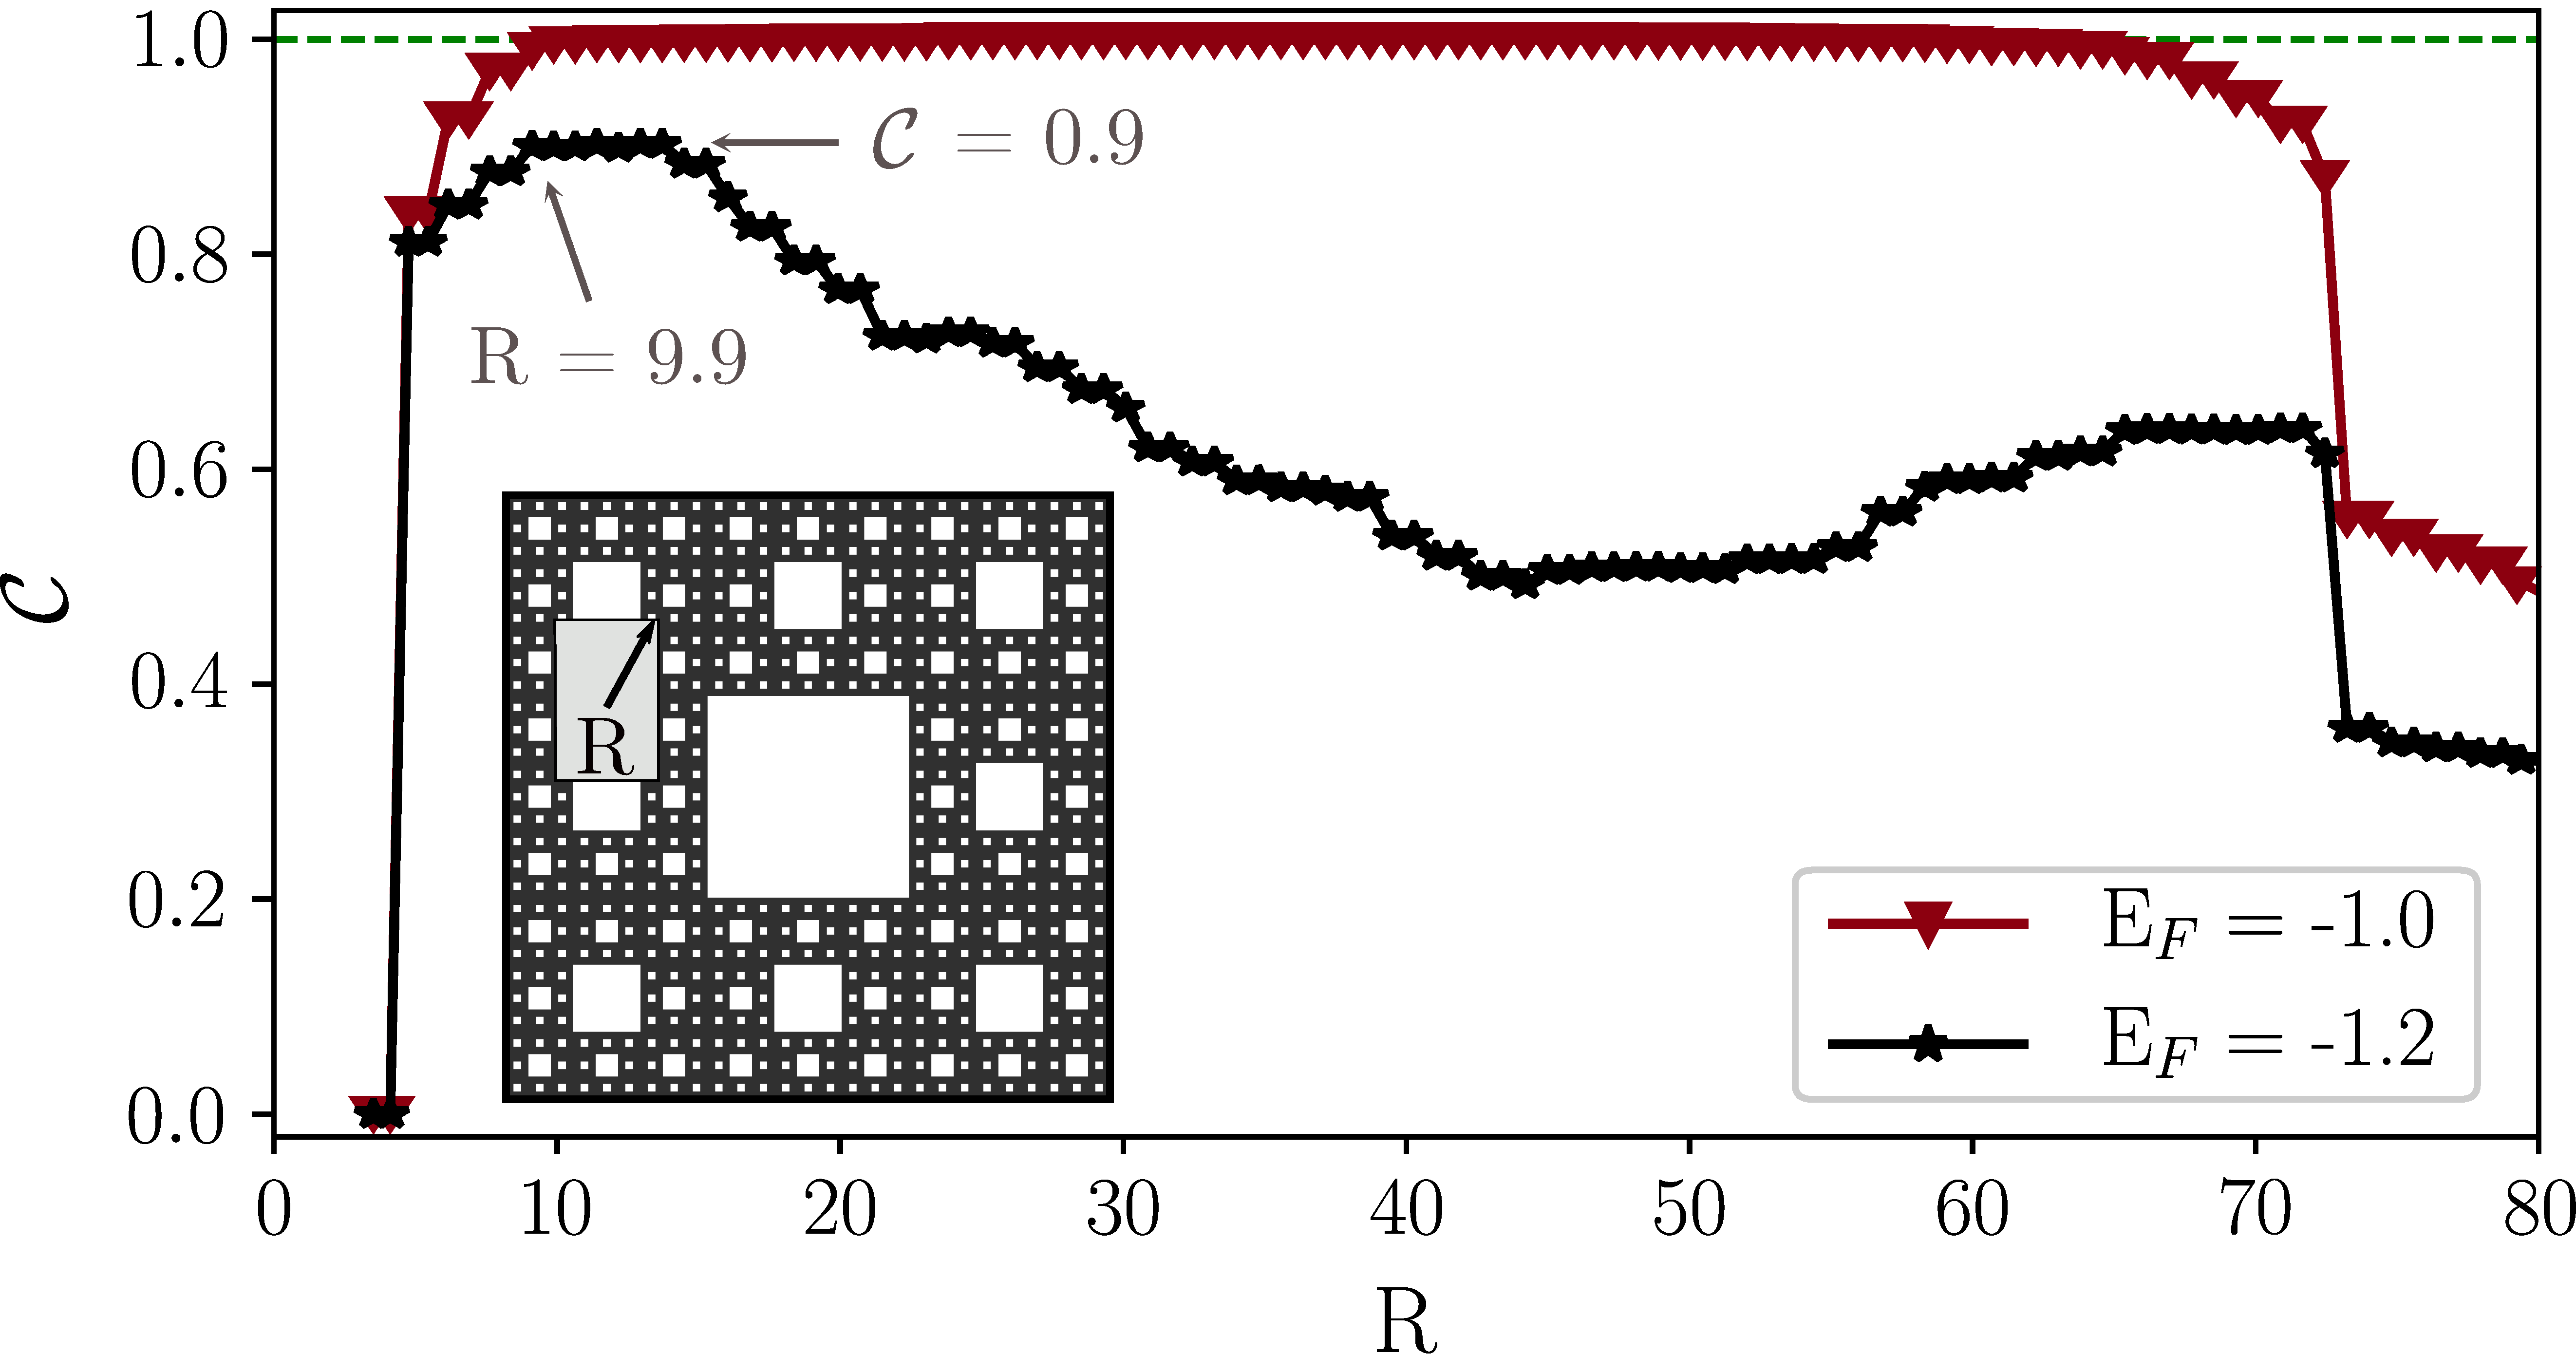
\includegraphics[width =0.8\columnwidth]{frac_chern_scaling.pdf}
\caption{\textbf{Scaling of the Chern number with respect to a real-space patch size:} Real-space Chern number calculations for Sierpiński carpet as a function of the half of the diagonal of a rectangular patch $R$ for two Fermi levels $E_F = -1.2$ and $E_F = -1.0$ at fixed flux $\alpha = 1/4$. For spectral regions exhibiting stable plateaus with quantized $\mathcal{C}$, this quantization is observed for a large range of patch sizes. In case of large DOS regions, in which we dominantly observe deviation from a quantized value of $\mathcal{C}$, the value of $\mathcal{C}$ is sensitive to the size and shape of the summation region. $R = 9.9$ corresponds to the size of the patch shown in Fig.~\ref{fig:lattice}~(a).}
\label{fig:ChernScaling}
\end{figure}

\section{Effect of disorder}
Topological matter is often defined in terms of robustness against disorder. For this reason, we would like to investigate the effect of disorder by adding extra term $\sum_i V_i c_i^{\dagger} c_i$ to the Hamiltonian in Eq.~\eqref{eq:frac_ham}, where $V_i$ is drawn from a uniform distribution $\left[ -W/2, W/2 \right]$ and $W$ corresponds to the disorder strength. If the system is characterized by a non-vanishing Hall conductivity, transition to a topologically trivial phase leads to localization of all states at some critical value of disorder, including the protected boundary modes. Disorder-induced topological phase transition is accompanied by a so-called levitation and pair annihilation mechanism~\cite{PhysRevLett.52.2304, onoda}. As the disorder increases, the states characterized by non-zero Chern number move towards each other, they meet at intermediate disorder values and annihilate, ultimately leading to Anderson localization at large disorder strength exceeding the band width.

This transition can be captured by level spacing defined as the difference between neighbouring energy levels. For a given energy $\epsilon$ and disorder realization $\{V_i\}$, we find two closest eigenvalues satisfying $ E_{\lambda, \{V_i\}} < \epsilon < E_{\lambda + 1, \{V_i\}}$, then calculate level spacings $s_{\epsilon, m, \{V_i\}} = E_{\lambda + m + 1, \{V_i\}} - E_{\lambda + m, \{V_i\}}$, where $m \in \lbrace -k, k \rbrace$, and normalize them. We set $k = 2$ as proposed in Refs.~\cite{2010:ProdanDisordCI, 2011:Prodan} and point out that incorporating differences between further neighbouring levels does not affect the results. Hence, we can study the distribution of the level spacings and the variance $\mathrm{Var} (s_{\epsilon}) = \langle s_{\epsilon}^2 \rangle - \langle s_{\epsilon} \rangle^2$ to determine whether states are localized or extended. The average is taken with respect $m$ and $10^3$ disorder realizations for fixed $\epsilon$. According to the random matrix theory, Hamiltonians with broken time-reversal symmetry are modelled by Gaussian unitary ensemble (GUE). If states are delocalized, then the level spacings should follow the Wigner-Dyson distribution $P_{\mathrm{GUE}} (s) = \frac{32 s^2}{\pi^2} e^{-\frac{4}{\pi} s^2}$ with the variance $\mathrm{Var}(P_{\mathrm{GUE}}) = 0.178$. Localized states, on the other hand, are expected to obey the Poisson distribution $P (s) = \exp (-s)$ with a large variance $ \sim \mathcal{O}(1)$. Consequently, we use the numerically obtained distribution of the level spacings for several disorder amplitudes $W$ to compute the variance in order to demarcate between localized and delocalized states.

Since disorder calculations require exact diagonalization of the Hamiltonian repeatedly, we consider here smaller systems (iteration $n = 4$ in case of SC and $n = 5$ for SG). This is justified by the fact that fractals exhibit same statistical properties at different scales. In Figs.~\ref{fig:frac_SC} (d) and \ref{fig:frac_SG} (d), we present the difference between $\mathrm{Var} (s)$ and $\mathrm{Var}(P_{\mathrm{GUE}})$ at fixed flux $\alpha = 0.25$. Regions in energy for which the Chern number is quantized are characterized by a large $\mathrm{Var} (s)$ at small values of $W$. There are two possible transition scenarios, which can be observed by following a line of increasing $W$ at constant energy, represented by white and blue arrows. Former case corresponds to a direct transition to fully localized system, without $\mathrm{Var} (s)$ ever becoming close to $\mathrm{Var}(P_{\mathrm{GUE}}) = 0.178$. In the latter case, a localized region at small $W$ is separated from the Anderson insulating limit by a delocalized region with $\mathrm{Var}(P_{\mathrm{GUE}}) = 0.178$. 

As a cross-check of our calculations, we compare the variances of the level spacings computed over the whole flux range at three different disorder strengths $W = 1, \, 3, \, 5$ for regular and fractal lattices (results are illustrated in Figs. \ref{fig:var_SC_square} and \ref{fig:var_SG_triangle}). In case of square and carpet, large variance exactly at $\alpha = 1/2$ is observed as systems become time-reversal invariant.

\begin{figure}[h]
\centering
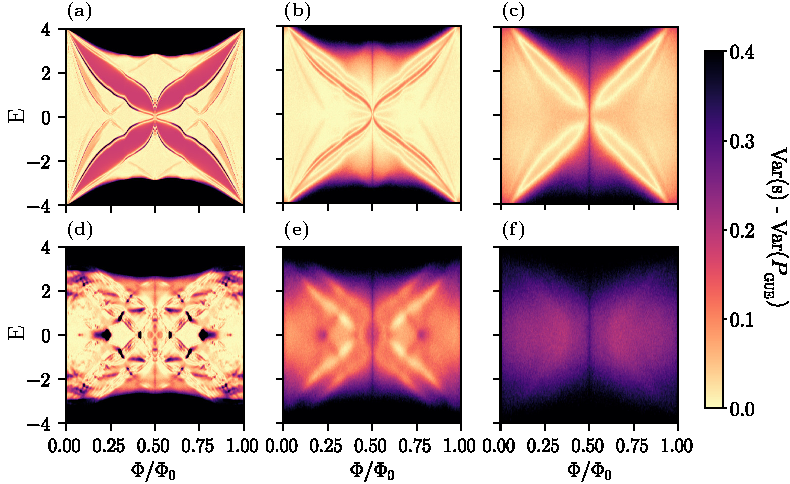
\includegraphics[width=0.95\textwidth]{frac_square_sc.pdf}
\caption{\textbf{Variance of the level spacings for (a, b, c) a square lattice and (d, e, f) the Sierpiński carpet:} variances in the energy - flux plane at three disorder strengths, \textbf{(a, d)} $W = 1$,  \textbf{(b, e)} $W = 3$, and \textbf{(c, f)} $W = 5$.} 
\label{fig:var_SC_square}
\end{figure}

\begin{figure}[h]
\centering
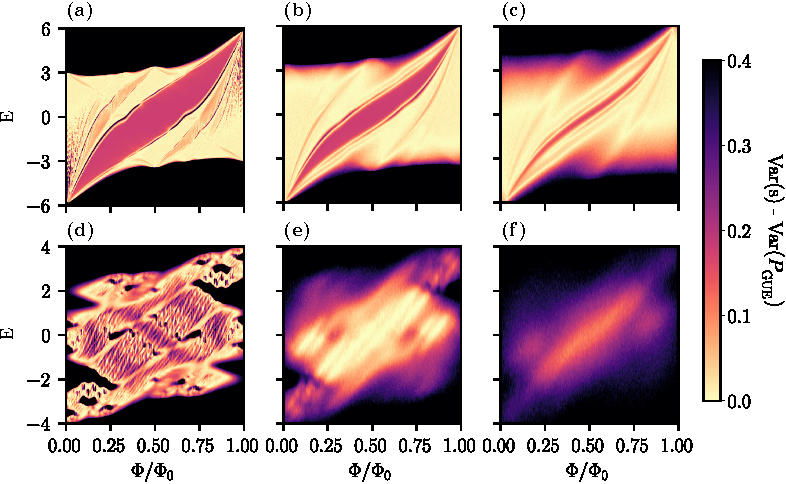
\includegraphics[width = 0.95\columnwidth]{frac_triangle_sg.pdf}
\caption{\textbf{Variance of the level spacings for (a, b, c) a triangle lattice and (d, e, f) the Sierpiński gasket:} variances in the energy - flux plane at three disorder strengths, \textbf{(a, d)} $W = 1$,  \textbf{(b, e)} $W = 3$, and \textbf{(c, f)} $W = 5$.}
\label{fig:var_SG_triangle}
\end{figure}